\chapter{系统前端设计与优化}
本章节主要介绍对本系统前端采用的特殊设计以及采用的原因及实现。

在本章中将会介绍两个特殊的设计:

1. 系统前端包含一个数据库

2. 系统前端提出了一层新抽象:表决计算精度

下面将详细讲解采用此类设计的原因及实现。

\section{前端数据库}

\subsection{设计原因}

系统前端包含一个数据库的设计来源于本系统的具体业务需求。本视频表决会议系统的目的是为了实现破产领域全流程线上办公的表决会议模块能够满足需求,对本系统来说,简化管理人的工作是核心目的。

在视频表决会议系统中,总共有三种用户,一种是管理人用户,一种是债权人用户,还有一种是其他参会人员用户。对于债权人用户和其他参会人员用户相关的功能来说,会议相关的数据请求量都很小,对于采取前端数据库方案起决定性因素的是管理人用户的功能。管理人用户有参看参会详情、查看会议详情和查看表决详情的功能,对于一个会议来说,这三个功能的数据综合起来可以囊括此会议的全量数据,而在会议进行过程中,这三个功能的数据是从 WebSocket 服务全量返回的,因此相当于在前端保存了全量的数据。

在前端拥有全量数据的情况下,可以在前端维护一个数据库,将管理人功能部分的计算交由前端进行,这样可以变相减少后端的压力。如果要将计算前后端区分完整,目前的设计下需要的代码量远远超过将计算交由前端进行,并且代码的维护会比较困难,另外前端数据库的设计是将 Redux 类比成后端数据库设计的,如果要把计算迁移到后端,可以在现有的前端计算代码上做快速迁移。因此,本系统采取了前端数据库的设计。

\subsection{存储设计}

确定了前端数据库的设计后,接下来需要考虑的是前端数据库的具体设计实现。

要实现将 Redux 作为一个数据库,首先要考虑所有实体数据的存储问题。此处以议程实体 Schedule 为例,要将所有的 Schedule 数据存入 Redux中。 如果仅仅凭借原生 JS 的方法,最容易想到的两种存储方式,一是通过数组 Array 进行存取,一种是通过对象 Object 进行存取。

首先考虑使用数组 Array 进行存储。

\subsubsection{Array 存储}

{\setmainfont{Courier New Bold}
\begin{lstlisting}
  const scheduleArr: ReduxSchedule[] = []
 \end{lstlisting}}
为了考虑使用 Array 存储是否可取,假设存在这样一种情况,有 1000 个 Schedule 发生了更新,对于用 Array 存储的 Schedule 来说,Redux 要扫描数组 1000 次,每次更新一个数据。

即如果总的议程 Schedule 数量为 N,发生更新的 Schedule 数量为 M,用 Array 存储的情况下,更新 M 条 Schedule 数据的时间复杂度是 O(N*M)。这个时间复杂度是不可接受的,因此直接用 Array 存储的方式是不可取的。

在用 Array 存储的方式不可取的情况下,考虑使用原生 JS 的另一种存储方式, 使用 Object 存储。

\subsubsection{Object 存储}

{\setmainfont{Courier New Bold}
\begin{lstlisting}
  const scheduleObj: Record<string, ReduxSchedule> = {}
 \end{lstlisting}}
为了考虑使用 Object 存储是否可取,仍然假设这样一种情况,有 1000 个 Schedule 发生了更新,在使用 Object 存储的情况下,更新每个 Schedule 的复杂度都是 O(1), 因此总的时间复杂度变成了 O(M)。

O(M) 的时间复杂度似乎能满足要求,但实际上 Object 每次的 O(1) 级别的更新都非常慢,因为 Object 的实现虽然接近哈希表,但 JS 并不期望它内部存海量数据,也不希望将 Object 当作哈希表进行使用。在存海量数据的情况下,Object 的性能会比起存储少量数据的 Object 慢几十倍,并不能完全满足系统的需求,因此直接使用 Object 存储的方式也是不可取的。


直接使用原生JS的 Array 和 Object 都不能满足需求的情况下, 考虑使用其他结构进行存储。最容易想到的就是哈希表,通过查阅资料,考虑使用在 ES6 中提出的数据结构 Map 。

\subsubsection{Map 存储}

对于在 ES6中提出的数据结构 Map ,无论存储数据的量级大小,性能的变化幅度都并不大,存取大量的数据也和存储少量数据相比性能都比较高。将 Map 和 Object 进行对比, 同等条件下 Map 比 Object 快 2.38 至 80 倍,时间复杂度保持在 O(M) 的级别, Map 的使用见下方代码展示。

{\setmainfont{Courier New Bold}
\begin{lstlisting}
  // 初始化一个 map, key 是 scheduleId, value 是 ReduxSchedule 实体
  const scheduleMap: Map<number, ReduxSchedule> = new Map()
  scheduleMap.set(12, '对应的 schedule 实体')
  console.log(scheduleMap.get(12))
  // 打印结果:'对应的 schedule 实体'
 \end{lstlisting}}

  使用 Map 进行存储解决了查询和更新的性能问题, 但是在使用 Map 的过程中,发现了另一个问题,满足渲染要求带来的性能损耗过大。

  React的渲染机制要求,所有数据必须是不可变的,只要状态数据 setState() 前后的数据满足:
  \begin{equation}
    (prev, curr) => (prev === curr)
  \end{equation}
  的条件,前端组件就不会触发页面渲染。

  在这种情况下,不管是使用 Array 、 Object 还是 Map ,在触发 Schedule 更新的时候,除了更新 M 条新的 Schedule 数据以外,还需要将原本的 N 条 Schedule 数据重新复制一遍,生成一个新的数据结构,而这样做的目的仅仅是为了触发 React 的渲染机制:

  \quad{}a. Array 的更新渲染时间复杂度是 O(N*M + N)


  \quad{}b. Object 的更新渲染时间复杂度是 O(M + N)


  \quad{}c. Map 的更新渲染时间复杂度是 O(M + N)

  在以上三种存储方式都不能满足需求的情况,经过进一步调研发现,使用 Immutable.JS 能够解决上述问题。

  \subsubsection{Immutable.JS}
  Immutable.JS 由 Facebook 工程师 Lee Byron 花费 3 年时间打造,与 React 同期出现,但没有被默认放到 React 工具集里(React 提供了简化的 Helper)。它内部实现了一套完整的 Persistent Data Structure,还有很多易用的数据类型。本系统选择使用了Immutable.JS 的 Map 数据结构。

  Immutable.Js 的 Map 数据结构对应于 ES6 的 Map 对象,通过使用 Map 数据结构可以解决查询和更新的性能问题。另一个需要解决的问题是由于 React 渲染机制在更新的时候需要重新复制一次数据结构所带来的损耗,而 Immutable.Js 使用的 Structural Sharing(结构共享)的方式可以解决这个问题。

Immutable 中文意义为不可变的,Immutable Data 就是一旦创建,就不能再被更改的数据。对 Immutable 对象的任何修改或添加删除操作都会返回一个新的 Immutable 对象。Immutable 实现的原理是 Persistent Data Structure(持久化数据结构),也就是使用旧数据创建新数据时,要保证旧数据同时可用且不变。同时为了避免 deepCopy 把所有节点都复制一遍带来的性能损耗,Immutable 使用了 Structural Sharing(结构共享),即如果对象树中一个节点发生变化,只修改这个节点和受它影响的父节点,其它节点则进行共享。

\begin{figure}[!htp]
    \centering
    \begin{subfigure}{0.4\textwidth}
      \centering
      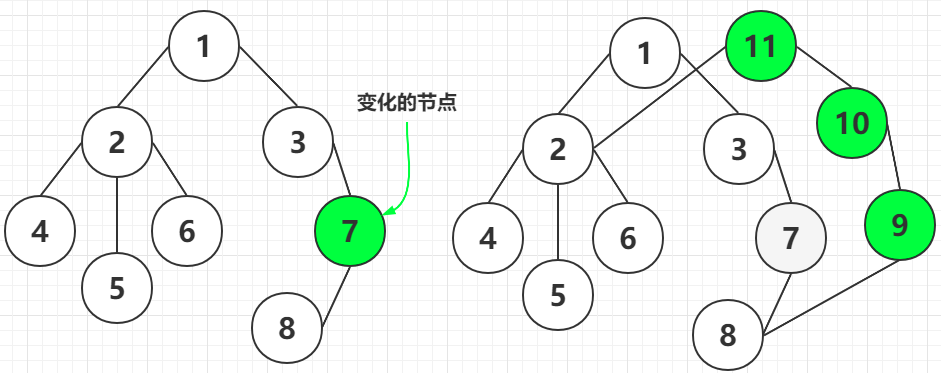
\includegraphics[height=4cm]{immutable1.png}
      \caption{}
    \end{subfigure}
    \hspace{1cm}
    \begin{subfigure}{0.4\textwidth}
      \centering
      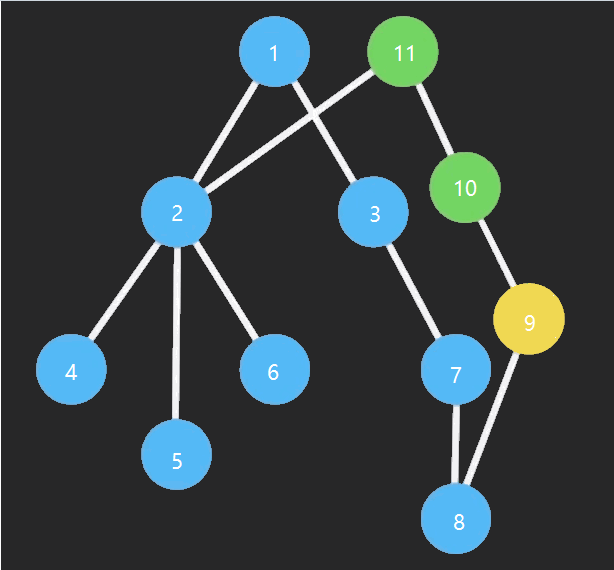
\includegraphics[height=4cm]{immutable2.png}
      \caption{}
    \end{subfigure}
    \begin{subfigure}{0.4\textwidth}
      \centering
      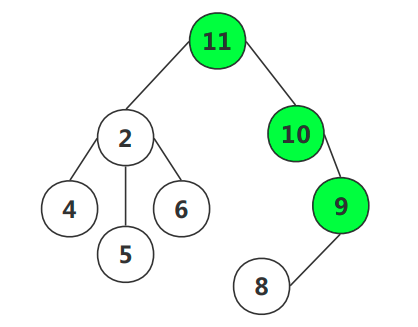
\includegraphics[height=4cm]{immutable3.png}
      \caption{}
    \end{subfigure}
    \caption{结构共享示意图}
    \label{fig:immutable}
  \end{figure}

  接下来通过一个例子介绍 Structural Sharing(结构共享),假设存在一个旧数据 oldData,它的对象树中有8个节点,如图~\ref{fig:immutable} (a)所示,现在对对象树中的节点7进行修改,这个操作将会返回一个新的 Immutable 对象。

   根据 Structural Sharing(结构共享)的原则,只修改节点7和受节点7影响的父节点,根据图~\ref{fig:immutable} (a) 可以看到受到影响的节点有节点1、节点2和节点7。对这三个节点复制一遍创建出新的节点9、节点10及节点11,节点9为节点7的复制,与原子节8相连,节点10为节点3的复制与节点7的复制节点9相连,节点11为节点1的复制,与节点1的子节点2和节点3的复制节点10相连,如图~\ref{fig:immutable} (b)所示,最后得到了一个新的Immutable 对象,如图~\ref{fig:immutable} (c)所示。

  根据前面说到的 React 渲染问题,如果使用 Map,直接更新 Map 并不能触发渲染,而使用ImmutableMap 则可以直接触发渲染,对比效果见下方代码展示。

  {\setmainfont{Courier New Bold}
  \begin{lstlisting}
    // 两种Map 的 key 都是 scheduleId, value 都是 ReduxSchedule 实体
    // ES6 Map
    const scheduleMap: Map<number, ReduxSchedule> = new Map()
    scheduleMap.set(12, '对应的 schedule 实体')
    const newMap = scheduleMap.set(14, '另一个 schedule 实体')
    console.log(scheduleMap === newMap)
    // 打印结果:true

    // ImmutableMap
    const scheduleMap: ImmutableMap<number, ReduxSchedule> = new ImmutableMap()
    scheduleMap.set(12, '对应的 schedule 实体')
    const newMap = scheduleMap.set(14, '另一个 schedule 实体')
    console.log(scheduleMap === newMap)
    // 打印结果:false
   \end{lstlisting}}

  通过使用 Immutable.js,触发渲染的性能表现如下:

  \quad{}a. Immutable.Array 的渲染时间复杂度是 O(N*M)

  \quad{}b. Immutable.Map 的渲染时间复杂度是 O(M)

  前端 Redux 通过使用 ImmutableMap,将 Redux 实现成了一个数据库,只要 Redux ImmutableMap 发生了变更,前端就触发使用该 ImmutableMap 的组件的渲染。

  \subsection{其他问题}
  在将前端 Redux 实现为一个数据库的过程中,还有一些问题凸显了出来,这里介绍两个本系统的重要问题及解决方法或思路。

  第一个问题是在将前端 Redux 实现为数据库的过程中,由于各个数据之间存在有关系,例如议程 Schedule 有对应的表决组 Groups,表决Ticket 有对应的会议债权人 MeetingCreditor,这之间的对应关系的存储问题。

  目前的设计实现是实体与另一类实体的关系用外键存储,原因是只有这样才能正确触发渲染。假设在Redux数据库存储的议程实体 Schedule 中,groups 字段是一个数组,它保存了和 Schedule 相关的表决组。
  如果存的是表决组 Object ,那么表决组 Map 发生改变后,由于 groups 数组没有发生改变,用到 groups 字段的组件就无法触发渲染。
  如果存的是表决组外键,那么表决组 Map 发生改变后,由于用到 groups 数组的组件一定会用到表决组 Map,那么用到 groups 字段的组件就能正常触发渲染。

  第二个问题Immutable.js 官方并不建议混用 Immutable.js 和原生 JS 对象,但是在本系统的 Redux 中混用了,采取混用方案的原因有如下两点:

  \quad{}a. Immutable.js 具有侵入性,官方要求为避免混淆,所有 Object 要么全用原生 JS 要么全用 Immutable.js,如果要在 Redux 中全套换用 Immutable.js,必须将 Redux 中的 combineReducer 组件全量替换,这就会和 Storage Middleware (存储中间件) 不兼容,导致所有其他用到 Redux 的组件都会出现问题,例如设置鉴权的 token header。


  \quad{}b. 在本系统设计中,使用 Immutable.Js 只是借用其高性能的 ImmutableMap 的能力。而一旦将 Immutable.js 的数据结构作为业务数据,项目代码的可复用性就会变得非常差,并且无论之后进行前端做优化还是计算向后端迁移,项目代码都会变得非常难维护。在设计中ImmutableMap 只是起到像数据库一样的查询作用,所以本次设计尽量缩短 Immutable.js 库的使用范围,避免在业务逻辑用到的数据结构中使用 Immutable.js 的数据结构。

  另外前端的计算工作并不是全写死的,本系统的优化方向可以分为两类:

  \quad{}a. 前端进行优化,提升 QPS 至万级别。

  \quad{}b. 前端的计算向后端迁移。

  无论进行哪种优化,都能解决掉 Immutable.js 所解决的“渲染不触发”的问题,完成两种优化中任一种都可以在之后将 Immutable.js 去掉。

  \section{表决计算精度}
  \subsection{什么是表决计算精度}
  表决计算精度是表决前端提出的一层新的抽象,表决计算精度的定义:

  \quad{}a. 表决计算精度指的是一个议程的表决通过方式的计算精度,即指明一个议程通过与否的条件是各个表决组都得通过,还是不考虑表决组,只要议程通过即可。


  \quad{}b. 表决计算精度的概念只在需要表决的议程下出现。无需表决议程没有表决计算精度。

  表决计算精度是议程的一个字段,名称为 highPrec (boolean) 目前只在 Redux 中存在。另外表决计算精度会影响债权人、债务人表决相关的业务逻辑,进而影响前端的渲染。

  \subsection{为什么需要表决计算精度}

  首先,因为项目现在表决类型是Hard Code (硬编码),并不是一个变量。如果这部分的业务需求发生了变化,本系统的整个架构设计从持久层,到后端,到实时表决端,再到前端,以及接口端全部都得重修修正。一个直观的例子,由于只有重整表决需要计算到表决组级别的特殊性,本系统现有接口的命名区分为 noReorgnization (非重整表决),reorgnization (重整表决),如果新增一个议题,表决计票方式同重整表决,但命名叫新式表决,那么原本的命名 noReorgnization,reorgnization 需要改成 noReorgnizationAndNew (非重整和新式表决), reorgnizationAndNew (重整和新式表决),以及其他相关的部分全部都需要修正。如果通过表决精度来进行区分,之后的修正只需要在前端只需要加个枚举常量就可以解决问题。

  其次表决计算精度决定了前端的渲染,有了表决精度的划分,前端渲染的代码逻辑会更加清晰。例如,债权人的投票表格中,不同表决精度的议程,投票表格的行单元格合并是不同的;管理人查看表决数据统计的时候,不同表决精度的议程,表决数据统计的行单元格合并是不同的;管理人查看表决详情时,不同表决精度的议程对应的表决详情是完全不同的两张表。
  
  以管理人查看表决详情为例,从业务逻辑出发,
  高精度议程表决详情的每一行,是选中表决组下的一个表决项 Ticket,如图~\ref{fig:reAndNoRe}(a)中第一行代表债权人上海启岚石油制品有限公司在审议A议程下普通债权中的表决金额为49349400.00元。
  低精度议程表决详情的每一行,是该议程下的一个会议债权人 MeetingCreditor,如图~\ref{fig:reAndNoRe}(b)中第一行代表债权人上海启岚石油制品有限公司在审议A议程下总共的表决金额为49349400.00元。

  \begin{figure}[!htp]
    \centering
    \begin{subfigure}{0.45\textwidth}
      \centering
      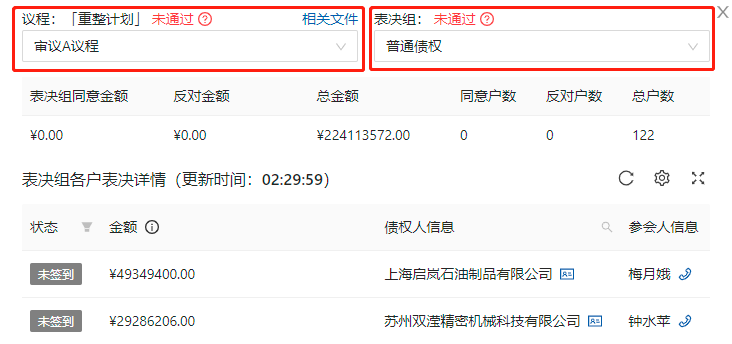
\includegraphics[height=4cm,width=7cm]{re.png}
      \caption{高精度议程表决详情}
    \end{subfigure}
    \hspace{1cm}
    \begin{subfigure}{0.45\textwidth}
      \centering
      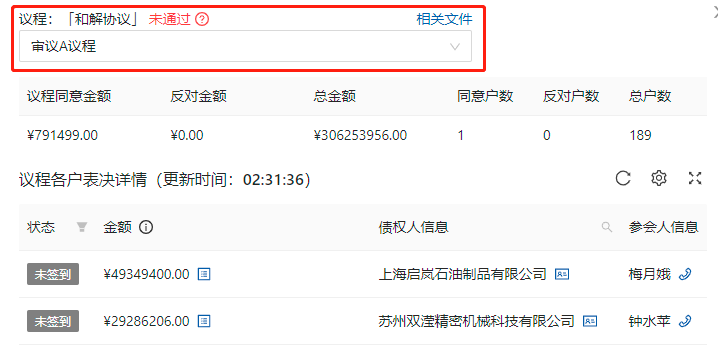
\includegraphics[height=4cm,width=7cm]{noRe.png}
      \caption{低精度议程表决详情}
    \end{subfigure}
    \caption{高精度和低精度对比图}
    \label{fig:reAndNoRe}
  \end{figure}

  总的来说,表决计算精度的提出,一是让业务代码可维护性变强了;
  二是让前端渲染逻辑更加清晰了。

  \section{Redux中的数据结构}

  在 Redux 中存储了基于 baseMeetingUser 的会议用户相关的数据结构 meetingAgent 和 meetingManager;存储了表决相关的数据结构 scheduleMap、meetingCreditorMap 和 groupMap。

  \subsection{会议用户相关的数据结构}

  \begin{figure}[!htp]
    \centering
    \begin{subfigure}{0.6\textwidth}
      \centering
      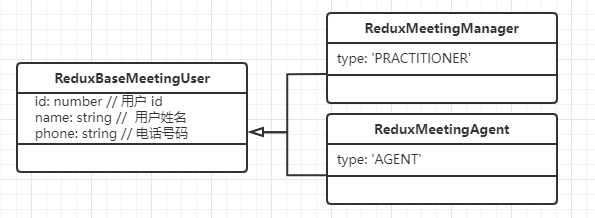
\includegraphics[height=4cm,width=10cm]{meetingUser.png}
      \caption{}
    \end{subfigure}
    \hspace{1cm}
    \begin{subfigure}{0.3\textwidth}
      \centering
      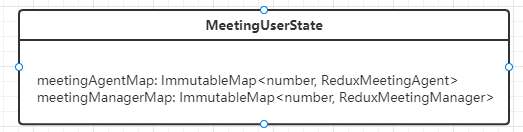
\includegraphics[height=2cm,width=6cm]{meetingUserState.png}
      \caption{}
    \end{subfigure}
    \caption{用户相关数据结构}
    \label{fig:meetingUser}
  \end{figure}

  meetingAgent 和 meetingManager 继承自 baseMeetingUser, baseMeetingUser 中包含信息用户Id,用户姓名和用户的电话号码。 meetingManager 的类型为 PRACTITIONER (管理人), meetingAgent 的类型为 AGENT (代理人),如图~\ref{fig:meetingUser}(a)。

  meetingUserState 中包含两个哈希表分别存储 meetingAgentMap 和
  meetingManagerMap 。 两个哈希表的键值对的键都是用户的ID号,值都是对应的 meetingAgent 和 meetingManager 实体,如图~\ref{fig:meetingUser}(b)。

  \subsection{表决相关的数据结构}

  scheduleType 是 Redux 中特别存储的议程类型,目的是为了方便快速地定位该议程的类型背后有关的表决信息,并由此决定前端的渲染,其中包含 name (议程类型名), description (议程类型描述), quotaPassRatio (金额通过比例), ticketPassRatio (票数通过比例), highPrecision (是否高精度),如图~\ref{fig:scheduleType}所示。

  \begin{figure}[!htp]
    \centering
    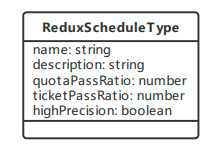
\includegraphics[height=3cm]{scheduleType.png}
    \caption{议程类型数据结构示意图}
    \label{fig:scheduleType}
  \end{figure}

  对于金额通过比例,若比率为负数,则意味着 “金额通过” 不考虑,对于精度到表决组的议程,该比率为 “各个表决组内通过金额” 的比率,对于精度到议程的议程,该比率为 “整个议程通过的金额” 的比率。

  对于票数通过比例,若比率为负数,则意味着 “票数通过” 不考虑,对于精度到表决组的议程,该比率为 “各个表决组内通过票数” 的比率,对于精度到议程的议程,该比率为 “选择通过的总债权人户数” 的比率。

  highPrecision (是否高精度)为计算精度。为 true 则意味着为高精度议程,即议程通过需要精确到各个表决组都通过,为 false 则意味着计算精度不高,只要议程下的总量数据通过即可,忽略表决组因素。另外,该字段会影响数据在前端的展示,目前只有 “重整计划” 议程是高精度的。

    \begin{figure}[!htp]
      \centering
      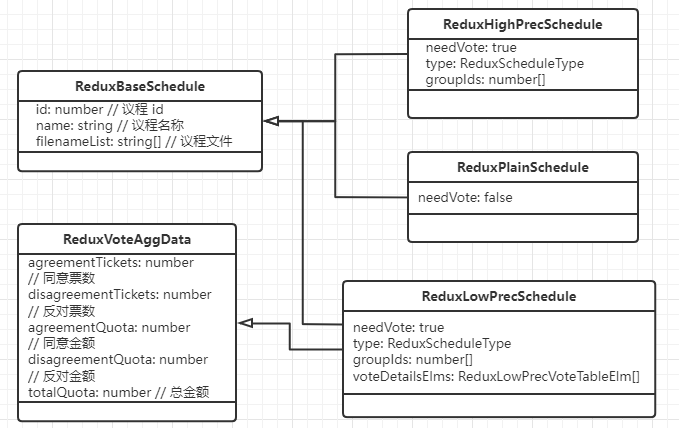
\includegraphics[height=10cm]{schedule.png}
      \caption{议程相关数据结构示意图}
      \label{fig:schedule}
    \end{figure}

    如图~\ref{fig:schedule}所示,对于表决议程来说,表决议程分为三种类型 highPrecSchedule (高精度表决议程)、lowPrecSchedule (低精度表决议程) 和 plainSchedule (普通议程)。以上三种类型议程均继承自 basicSchedule (基础议程), 基础议程中包含议程的ID号,议程的名称和议程的文件信息 (目前议程文件默认只有一个文件,即首文件)。

  plainSchedule (普通议程)即无需投票的议程,因此只在 basicSchedule (基础议程) 基础上多出了 needVote 属性,且值为 false,表示 plainSchedule (普通议程) 为无需投票的议程。

  highPrecSchedule (高精度表决议程) 即需要投票且投票精度到表决组级别的议程,在 basicSchedule (基础议程) 基础上多出了 needVote,type 和 groupIds 属性。needVote的值一定为 true,type 中 highPrecision 属性一定为 true, groupIds 用来存储和议程相关的所有表决组的ID号,高精度议程表决精确到表决组级别,因此 VoteAggData (表决复合数据) 在 group 级别。

  LowPrecSchedule (低精度表决议程) 即需要投票且投票精度到议程级别的议程,在 basicSchedule (基础议程) 基础上多出了 needVote,type,voteDetailsElms 和 groupIds 属性。needVote的值一定为 true,type 中 highPrecision 属性一定为 false, groupIds 用来存储和议程相关的所有表决组的ID号,voteDetailsElms 是低精度议程中,用于渲染 “表决详情” 的数据结构,每一项事实上是一个 meetingCreditor。低精度议程表决精确到议程级别,因此 VoteAggData (表决复合数据) 也在议程级别。

  VoteAggData (表决复合数据) 包含议程或表决组的表决情况,包含 agreementTickets (同意票数), disagreementTickets (反对票数), agreementQuota (同意金额), disagreementQuota (反对金额), totalQuota (总金额) 属性,用于展示议程或表决组的表决情况以及用于计算通过情况。

  \begin{figure}[!htp]
    \centering
    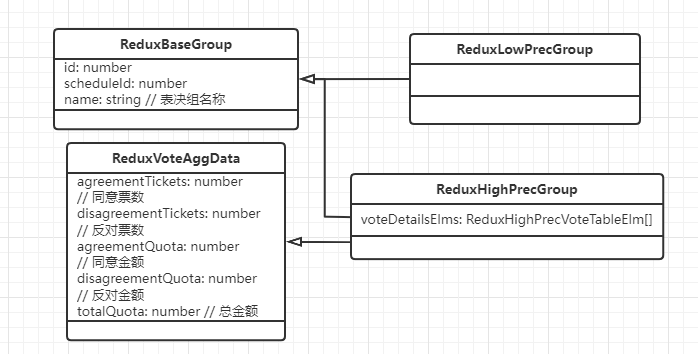
\includegraphics[height=8.5cm]{group.png}
    \caption{表决组相关数据结构示意图}
   \label{fig:group}
  \end{figure}

  如图~\ref{fig:group}所示,对于表决组来说,表决组分为两种类型 highPrecGroup (高精度表决组) 和 lowPrecGroup (低精度表决组) 。以上两种类型议程均继承自 basicGroup (基础表决组), 基础表决组中包含表决组的ID号,表决组的名称和表决组所属的议程ID。

  对于highPrecGroup (高精度表决组) 来说,由于高精度议程表决精确到表决组级别,因此VoteAggData (表决复合数据) 也在表决组级别,另外还包含 voteDetailsElms 属性,高精度议程中,用于渲染 “表决详情” 的数据,每一项事实上是一个 ticket。高精度下,各表决组 “总票数” 为该 map 的 size 大小。

  对于lowPrecGroup (低精度表决组) 来说,由于低精度议程会忽略表决组级别,因此低精度表决组只需保存基础表决含有的信息即可。

  \section{其他设计}
  在原本的设计中,会议页面中所有的 view state (视图状态)散落于各个组件内部,各个组件用到了表决服务的各种数据,其请求方法离散地分布在各个组件内部,这会让实时表决服务接入时发生以下问题:

  \quad{}a. 实时表决的 client scaffold (客户端支架)并非 useHooks 风格,实际上是 class,其所有的后端请求型数据对应的 handler 必须在该 class 初始化时设定好,且无法接受后续状态更新。也就是说,如果现有的组件保持原样,所有的组件都需要传入一个 realtimeUpdate 函数,在管理人会议页面中将至少 11 个函数组合在一起,置入 handler 中,以便于在表决后端传来请求型消息时更新各级子组件内部的 state,这会让代码非常不直观,难以维护。

  \quad{}b. 由于获取到的 client 生命周期很有可能是未准备好甚至已结束的,而 client 并非 useHooks 实现,各级子组件每次 state update 时并不会重新获取 client scaffold 的实体,而是保留老的引用。这很可能导致由部分组件由于加载的异步性,永远无法接收到后端传来的数据,也无法向后端发送数据。

  \quad{}c. 本系统前端要根据当前是否在实时表决的信息来让各个子组件的请求决定走向 SpringBoot后端还是实时服务。这个状态在各个子组件中分别做判断和共享非常麻烦且很容易遗漏,无论是 试用 redux 还是 context 或者将这个 state 以 props 传给所有人,都要进行大量的编码。这意味着,即使用 useHooks 实现 client scaffold,也难以保证目前组件状态更新的健壮性和可维护性。

  基于以上的考虑,本系统进行了前端组件的表决状态提升设计,即将管理人与债权人的会议页面下表决组件的各级子组件状态提升至父组件,使数据流更新清晰明了,具体实现如图~\ref{fig:state}所示。

  \begin{figure}[!htp]
    \centering
    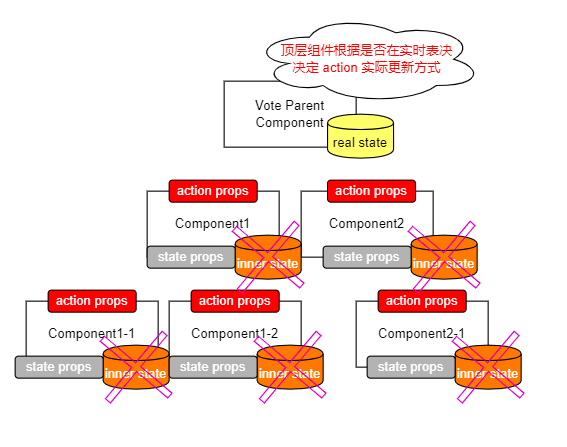
\includegraphics[height=8cm]{state.png}
    \caption{表决状态提升示意图}
   \label{fig:state}
  \end{figure}

  最顶层的组件中存有所有组件需要的真正 state,在上图中为亮黄色,数据为 SpringBoot后端 和 实时表决端拿到的复合数据。

  对于各级子组件,如果有表决相关的内部 state,将其定义为 inner state,全部删除。

  对于需要向后端请求数据的组件,将这个函数定义为 action,将它作为 props,由顶层组件级级传入。这意味着这部分数据的更新让顶层组件决定。action props 在图中显示为鲜红色。

  对于完全由 real state 决定的 state,直接将其作为 props 传入即可。这部分 props 在图中为深灰色。

对于实时表决时期,real state 只在第一次 action 触发时向 SpringBoot 后端获取数据,接下来这些 real state 都会接受实时数据的更新,

对于非实时表决时期,所有的 action 都将被设定为跳过从实时表决后端获取实时数据,直接从 SpringBoot 后端获取数据。